\documentclass[russian, utf8, pointsubsection, floatsubsection,
equationsection, emptystyle, simple]{eskdtext}
\usepackage[T2A]{fontenc}
\usepackage{eskdtotal}
\usepackage[math]{pscyr}
\usepackage{amssymb, amsmath, amsfonts, latexsym, amstext}
\usepackage{url}
\usepackage{multirow}
\usepackage{rotating}
\usepackage{ulem}
\usepackage{setspace}
\usepackage{graphicx}
\usepackage{longtable}
\usepackage{pdflscape}
\ESKDsectStyle{section}{\Large\bfseries}
\graphicspath{{pictures/}}

\usepackage{geometry}
\geometry{top=2cm}
\geometry{bottom=3.5cm}
\geometry{left=3.0cm}
\geometry{right=2cm}
\geometry{footskip=1.5cm}
\usepackage{fancyhdr}
\pagestyle{fancy}
\fancyhf{}
\renewcommand{\headrulewidth}{0pt}
\fancyfoot[C]{\thepage}

\usepackage{listings}
\lstset{language=C++,
  frame = ltrb,
  framesep = 5pt,
  basicstyle = \small\ttfamily,
  keywordstyle = \bfseries, 
  extendedchars = \true,
  identifierstyle = \bfseries\itshape, 
  commentstyle = \itshape,
  % stringstyle = \itshape, 
  numbers = left, 
  numberstyle = \scriptsize,
  breaklines = true,
  showspaces = true,
  showstringspaces = true
}
\renewcommand{\lstlistingname}{Листинг}

\ESKDtitle{Разработка политики ИБ ИС организации}
\ESKDdocName{Курсовая работа}
\ESKDsignature{ПГУ~3.090106.001}
\ESKDauthor{Захаров~М.\,А.}
\ESKDchecker{Алексеев~С.\,В.}
\ESKDnormContr{Алексеев~С.\,В.}
\ESKDcolumnIX{Гр.~06УИ1}
\addto\captionsrussian{\def\refname{Список использованных источников}}

\usepackage[unicode]{hyperref}
\hypersetup{pdfkeywords = ОПОИБ Алексеев}

\begin{document}
\ESKDthisStyle{empty}
\newpage
\begin{center}
  \begin{singlespace}
    Министерство образования и науки РФ  \\
    Государственное образовательное учреждение высшего профессионального образования \\
    \vspace{0.25cm}
    <<ПЕНЗЕНСКИЙ ГОСУДАРСТВЕННЫЙ УНИВЕРСИТЕТ>> \\
    \medskip 
    \hrule height 1pt
    \vskip 1pt 
    \hrule
    \vskip 3pt
    Кафедра <<Информационная безопасность систем и технологий>>
  \end{singlespace}

  \vspace{8em}

  \textsc{\textbf{РАЗРАБОТКА ПОЛИТИКИ ИНФОРМАЦИОННОЙ
    БЕЗОПАСНОСТИ ИНФОРМАЦИОННОЙ СИСТЕМЫ ОРГАНИЗАЦИИ}}\\[0.5cm]

  Пояснительная записка к курсовому проекту \\
  по дисциплине <<ОПОИБ>>\\[0.5cm]

  ПГУ 3.090106.001 ПЗ

  \vspace{8em}

  \begin{tabular}[h]{p{7cm}r}
    Руководитель КР,  & \\
    доцент & \underline{\hspace{3cm}}Алексеев~В.\,М.\\
    Исполнитель КР,  & \\
    студент & \underline{\hspace{3cm}}Захаров~М.\,А.
  \end{tabular}

  \vspace{\fill}

  Пенза 2010 

\end{center}
\newpage

\begin{center}
  \Large{\textbf{РЕФЕРАТ}}
\end{center}

Отчёт \ESKDtotal{page}~с., 2~рис., 12~табл.,
\ESKDtotal{bibitem}~источников, \ESKDtotal{appendix}~прил.

ИНФОРМАЦИОННАЯ СИСТЕМА, УЯЗВИМОСТЬ, АКТУАЛЬНАЯ УГРОЗА, ОЦЕНКА РИСКА,
ПОЛИТИКА БЕЗОПАСНОСТИ

Объектом исследования является информационная система отделения фонда
социального страхования.

Цель работы~--- получение навыков анализа угроз и разработки политики
безопасности информационной системы организации на примере отделения
фонда социального страхования.

В процессе работы были идентифицированы объекты защиты в
информационной системе, актуальные угрозы для информационных ресурсов
отделения фонда социального страхования, разработана политики
информационной безопасности информационной системы отделения фонда
социального страхования.

В результате исследования была разработана политика информационной
безопасности информационной системы отделения фонда социального
страхования. \newpage

%%% Local Variables: 
%%% mode: latex
%%% TeX-master: "../TermWork_OPOIB"
%%% End: 

\tableofcontents
\newpage
\begin{singlespace}
\hfill\parbox{6.5cm}{<<Утверждаю>>\\
  Зав. кафедрой ИБСТ\\
  \hbox to 6.5cm{\hrulefill С.\,Л.\,Зефиров}\\
  \def\hrf#1{\hbox to#1{\hrulefill}}
  <<\hrf{2em}>> \hrf{6em} \the\year~г.}	
	
\begin{center}\textbf{\normalfont\bfseries\large ЗАДАНИЕ}\\\textbf{на
    курсовую работу}\end{center}

по теме: \textbf{\uline{<<Разработка политики информационной
    безопас\-ности инфор\-мационной системы организации>>\hfill\quad}}

  \textbf{1 Дисциплина} \uline{\qquad Организационно-правовое обеспечение
    ин\-формационной безопасности\hfill}

  \textbf{2 Вариант задания} \uline{\qquad Организация~--- отделение фонда
    соци\-ального страхования. Исходный перечень угроз: нарушение
    конфиден\-циальности защищаемой информации, нарушение целостности
    защи\-щаемой информации. Уровни инфраструктуры: сетевых
    приложений, операционных систем\hfill}

  \textbf{3 Студент} \uline{\qquad Захаров М.\,А.\qquad }
  \textbf{группа} \uline{\qquad 06УИ1\hfill}

  \textbf{4 Исходные данные на проектирование}

  \uline{Должны быть разработаны описание бизнес-функций отделения
    фонда социального страхования, структура и схема информационных
    потоков её информационной системы с определенными топологией,
    количеством рабочих станций, объектами защиты.\hfill\quad}

  \uline{Должны быть разработаны описание угроз безопасности
    инфор\-мационной системы и сценарии их реализации. Описания угроз
    и источников угроз должны соответствовать модели ГОСТ Р ИСО/МЭК
    15408.\hfill\quad}

  \uline{Должны быть оценены риски реализации угроз для полного
    перечня угроз и определены актуальные для информационной системы
    угрозы.\hfill\quad}

  \uline{Должны быть сформулированы правила информационной
    безо\-пасности для противодействия угрозам информационной системы
    отде\-ления фонда социального страхования.\hfill\quad}

  \uline{Должна быть разработана политика информационной
    безопас\-ности информационной системы отделения фонда социального
    страхо\-вания на основе сформулированных правил.\hfill\quad}

  \textbf{5 Структура проекта}

  \textbf{5.1 Пояснительная записка (содержание работы):}

  \begin{itemize}
  \item \uline{описание информационных процессов организации,
      иденти\-фикация объектов защиты;\hfill\quad}
  \item \uline{структура информационной системы отделения фонда
      соци\-ального страхования и схема информационных
      потоков;\hfill\quad}
  \item \uline{анализ угроз информационным ресурсам;\hfill\quad}
  \item \uline{оценка рисков реализации угроз, выявление актуальных
      уг\-роз;\hfill\quad}
  \item \uline {разработка политики информационной безопасности
      инфор\-мационной системы отделения фонда социального
      страхова\-ния.\hfill\quad}
  \end{itemize}

  \textbf{5.2 Графическая часть}
  \begin{itemize}
  \item \uline{структура информационной системы отделения фонда
      соци\-ального страхования;\hfill\quad}
  \item \uline{схема информационных потоков в информационной системе
      отделения фонда социального страхования.\hfill\quad}
  \end{itemize}

  \textbf{6 Календарный план выполнения проекта}

  \textbf{6.1 Сроки выполнения работ по разделам:}

  \begin{itemize}
  \item \uline{утверждение ТЗ \hfill} к \uline{22.02.\the\year~г. }
  \item \uline{идентификация объектов защиты \hfill} к
    \uline{08.03.\the\year~г.}
  \item \uline{идентификация актуальных угроз \hfill} к
    \uline{12.04.\the\year~г.}
  \item \uline{разработка политики ИБ \hfill}
    к \uline{19.04.\the\year~г.}
  \item \uline{оформление и проверка отчёта о КР \hfill}
    к \uline{10.05.\the\year~г.}
  \item \uline{подготовка к защите курсовой работы\hfill} к
    \uline{24.05.\the\year~г.}
  \end{itemize}
  \hbox to 11cm {Дата защиты проекта \uline{\hfill \the\year~г.}}
  Руководитель работы \uline{\hfillАлексеев~В.\,М.}\\
  \hbox to 11cm {Задание получил \uline{\hfill8 февраля \the\year~г.}}\\
  Студент    \uline{\hfillЗахаров~М.\,А.}\\
  Нормоконтролёр    \uline{\hfillАлексеев~В.\,М.}\\
\end{singlespace}
\newpage

%%% Local Variables: 
%%% mode: latex
%%% TeX-master: "../TermWork_OPOIB"
%%% End: 

\newpage

\begin{center}
  \Large{\textbf{ВВЕДЕНИЕ}}
\end{center}
\addcontentsline{toc}{section}{Введение}

Информация~--- это имущество (или активы), которое, подобно другим
важным деловым активам, имеет ценность для организации и,
следовательно, должна быть защищена соответствующим
образом. Конфиденциальность, целостность и доступность информации
могут быть существенными аспектами для поддержания
конкурентоспособности, денежного оборота, доходности, юридической
гибкости и коммерческого имиджа. Информационная безопасность защищает
информацию от широкого диапазона угроз как раз для того, чтобы
обеспечить уверенность в непрерывности бизнеса, доведения до минимума
ущерба, наносимого бизнесу, и доведения до максимума возвращения
инвестиций и возможностей бизнеса.

Информационная безопасность достигается реализацией соответствующего
множества средств управления, которые могут быть \linebreak представлены
политиками, методами, процедурами, организационными структурами и
функциями программного обеспечения. Эти средства управления необходимо
устанавливать таким образом, чтобы обеспечивать уверенность в том, что
определенные цели безопасности организации достигнуты~\cite{1}.

Данная курсовая работа посвящена анализу информационной системы
отделения фонда социального страхования и по его результатам
разработана спецификация требований, призванных обеспечивать
руководство организации управлением и поддержкой информационной
безопасности, т. е. политика информационной безопасности.

Курсовая работа состоит из 3 разделов.

В первом разделе происходит идентификация объектов защиты в
информационной системе отделения фонда социального страхования.

Во втором разделе рассматриваются наиболее актуальные угрозы для
информационных ресурсов отделения фонда социального страхования.

Третий раздел посвящён разработке политики информационной безопасности
организации.

\newpage

%%% Local Variables: 
%%% mode: latex
%%% TeX-master: "../TermWork_OPOIB"
%%% End: 

\section{Идентификация объектов защиты в
  информационной системе фонда
  социального страхования}

\subsection{Цели и задачи фонда}

\point Цель деятельности фонда социального страхования~--- обеспечение
обязательного социального страхования граждан России.

\point Отделение фонда социального страхования осуществляет:

\begin{itemize}
\item выплату пособий по временной нетрудоспособности;
\item выплату пособий в связи с материнством и детством;
\item обеспечение социальными пособиями на погребение;
\item санаторно-курортное лечение. Оздоровление детей;
\item финансирование проведения углубленных медицинских осмотров
  работников занятых на работах с вредными и (или) опасными
  производственными факторами.
\end{itemize}

\point Функции фонда, которые могут быть автоматизированы с помощью
информационной системы: \label{functions}

\begin{enumerate}
\item организация банков данных по всем категориям страхователей;
\item ежеквартальный приём и выверка отчётных данных страхователей.
\end{enumerate}

\subsection{Идентификация информационных процессов}

В соответствии с функцией а) пункта~\ref{functions} можно
идентифицировать следующие информационные процессы.

\point Физическое или юридическое лицо, желающее зарегистрироваться в
качестве страхователя, отправляет с курьером (представителем
страхователя) на бумажном носителе заявление на регистрацию,
необходимые данные, а также документы, подтверждающие сферу
деятельности и уплату всех соответствующих налогов.

Получателем данной информации является специалист подразделения фонда,
ответственный за регистрацию страхователей.

\point На основе документов, предоставляемых физическим или
юридическим лицом, желающим зарегистрироваться в качестве
страхователя, специалист подразделения фонда, ответственного за
регистрацию страхователей (оператор), заносит необходимую информацию в
реестр (базу данных), добавляя к ней регистрационный номер и код
подчиненности. После чего с документов снимаются копии, которые вместе
с заявлением на регистрацию сдаются в архив. Подлинники документов
возвращаются страхователю.

\point Оператор получает доступ к информации, предоставленной
страхователем, но имеет право лишь на ввод её в базу данных. После
того, как данные о страхователе будут сохранены и отправлены по ЛВС на
сервер БД, единственным обладателем права доступа и модификации этих
данных становится администратор БД. В последующем доступ к информации,
хранящейся в БД, осуществляется через АРМ сотрудниками Фонда в
соответствии с их должностными обязанностями.

\point Используемые программные приложения:

\begin{itemize}
\item программа для ввода данных о страхователе;
\item СУБД;
\item ОС.
\end{itemize}

\point Ввод информации осуществляется непосредственно на АРМ
оператора, последующая обработка и модификация~--- на АРМ
администратора баз данных.

Ввод данных с бумажных носителей в реестр, добавление регистрационного
номера и кода подчиненности осуществляется оператором вручную.

\point Путь перемещения информации в ИС: АРМ оператора~---
коммутатор~--- маршрутизатор~--- сервер БД.

\point Обработанная информация в виде структурированной БД хранится на
сервере БД, а также на сервере резервного копирования. Доступ к
информации в БД осуществляется средствами запросов СУБД с АРМ
сотрудников фонда в соответствии с их должностными полномочиями.

В соответствии с функцией б) пункта~\ref{functions} можно
идентифицировать следующие информационные процессы.

\point Отчётные данные поступают от страхователя с курьером
(представителем страхователя) на бумажном носителе или через интернет
(посредством электронной почты с использованием ЭЦП).

Отчёт исходит от бухгалтера страхователя к оператору ИС фонда.

\point Если отчёт поступает с курьером на бумажном носителе,
специалист фонда (оператор) на своём рабочем месте осуществляет ручной
ввод информации в базу данных (данные приводятся к формализованному
виду), которая хранится на сервере баз данных. После чего отчёт
сдается в архив.

\point Путь перемещения информации в ИС: АРМ оператора~---
коммутатор~--- маршрутизатор~--- сервер БД.

\point При получении отчёта по электронной почте на первом этапе
администратор ИБ на своем АРМ производит проверку соответствующих
реквизитов электронно-цифровой подписи. При подтверждении подлинности
распаковывает сообщение с помощью программы-упаковщика, в противном
случае~--- уничтожает пакет.

Затем по внутренней ЛВС производит отправку полученных данных
специалисту подразделения фонда, ответственного за бухгалтерский учёт
и отчётность (оператору).

Оператор на своем АРМ осуществляет проверку правильности заполнения
формы. В случае положительного результата проверки оператор производит
добавление полученного отчёта к базе данных, хранящейся на сервере БД.
В противном случае оператор посредством факса уведомляет отправителя,
что его отчёт не принят, указав причину. После чего непринятый отчёт
будет уничтожен.

\point Путь перемещения информации в ИС: почтовый сервер~--- АРМ
администратора ИБ~--- коммутатор~--- АРМ оператора~--- коммутатор~---
маршрутизатор~--- сервер БД.

\point Администратор ИБ не имеет прав на модификацию
информации. Оператор имеет доступ к данной информации, но имеет право
лишь на ввод её в базу данных. После того, как отчёт будет сохранен и
отправлен по ЛВС на сервер БД, единственным обладателем права их
модификации становится администратор БД. В последующем доступ к
информации, хранящейся в БД, осуществляется через АРМ сотрудниками
фонда в соответствии с их должностными обязанностями.

\point Используемые программные приложения:

\begin{itemize}
\item программа для ввода данных отчёта;
\item СУБД;
\item программа-упаковщик;
\item программа для проверки ЭЦП;
\item ОС.
\end{itemize}

\point Отчётные данные страхователя заносятся в базу данных
специалистом фонда или автоматически.

\point После обработки обработанная информация в виде
структурированной БД хранится на сервере БД, а также на сервере
резервного копирования. Доступ к информации в БД осуществляется
средствами запросов СУБД с АРМ сотрудников фонда в соответствии с их
должностными полномочиями.

\point Лицом, ответственным за функциональным состоянием аппаратных
компонентов в ИС фонда социального страхования, является системный
администратор.

\subsection{Структура ИС фонда}

\point Информационная система фонда состоит из следующих элементов:

\begin{enumerate}
\item серверная ферма:
  \begin{enumerate}
  \item почтовый сервер;
  \item сервер обработки, на котором установлена СУБД;
  \item сервер резервного копирования.
  \end{enumerate}
\item Автоматизированные рабочие места:
  \begin{enumerate}
  \item операторов;
  \item администратора БД (резервного копирования);
  \item администратора почтового сервера;
  \item администратора ИБ.
  \end{enumerate}
\item Сетевое оборудование:
  \begin{enumerate}
  \item коммутатор;
  \item маршрутизатор.
  \end{enumerate}
\end{enumerate}

\point Графическое изображение конфигурации системы представлено на рисунке:

\begin{figure}[h]
  \centering
  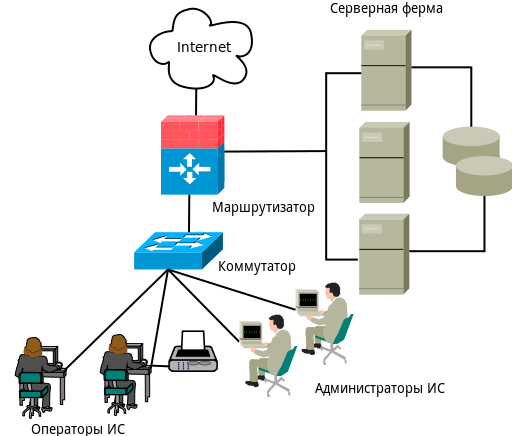
\includegraphics[width=\textwidth]{Structure}
  \caption{Конфигурация информационной системы фонда социального страхования}
  \label{fig:structure}  
\end{figure}

\subsection{Идентификация аппаратных ресурсов
  фонда как объектов защиты}

\point Следующим этапом курсовой работы является определение
ответственных за каждый аппаратный ресурс ИС и их полномочия по
отношению к этим ресурсам с точки зрения возможности изменения
конфигурации этих ресурсов. Для каждого аппаратного ресурса
определяются его пользователи и их полномочия тоже с точки зрения
возможности изменения конфигурации этих ресурсов, т.~е. происходит
идентификация аппаратных ресурсов как объектов защиты с указанием
возможных источников угроз для них.

\point Результат представлен в таблице~\ref{hardware} Приложения~\ref{AppendixA}.

\subsection{Идентификация информационных ресурсов
  фонда как объектов защиты}

\point На следующем этапе курсовой работы необходимо идентифицировать
информационные ресурсы, подлежащие защите.

\point В результате выполнения рабочих процессов организации
образуются следующие информационные ресурсы:

\begin{itemize}
\item документы, необходимые для регистрации страхователя, поступившие
  с курьером;
\item отчёт о работе страхователя, поступивший с курьером;
\item отчёт о работе страхователя, поступивший электронной почтой;
\item база данных.
\item резервная копия базы данных;
\end{itemize}

\point В таблице~\ref{tab:inf_resource} представлена классификация
информационных русурсов по степени критичности относительно
доступности, целостности и конфиденциальности.

\begin{table}[h]
\caption{Классификация ИР фонда по степени критичности}
\label{tab:inf_resource}
\small
\begin{tabular}{|p{5cm}|p{3cm}|p{3cm}|p{3cm}|}
\hline
\multirow{3}{4cm}{Информационный ресурс} & \multicolumn{3}{c|}{Степень
  критичности информации}\\\cline{2-4}
& Доступность & Целостность & Конфиденциаль\-ность \\\hline
Документы, необходимые для регистрации страхователя & Важная & Важная
& Значимая\\\hline
Отчётные данные страхователя на бумажном носителе & Важная & Важная &
Значимая \\\hline
Отчётные данные страхователя в электронном виде & Важная & Важная &
Значимая \\\hline
Содержимое сервера БД & Критическая & Критическая & Очень важная
\\\hline
Резервная копия БД & Важная & Очень важная & Очень важная
\\\hline
\end{tabular}
\end{table}
\normalsize

\point В таблице~\ref{infsource} Приложения~\ref{AppendixA} определяются
ответственные за информационные ресурсы фонда, их пользователи, а
также как ответственные и пользователи используют информационные
ресурсы.

\subsection{Схема информационных потоков в ИС фонда}

На основе результатов предшествующего анализа на базе структуры ИС
фонда разрабатывается схема информационных потоков в ИС фонда. Схема
информационных потоков представлена на рисунке~\ref{fig:infresurs}.

1 --- отчётные данные страхователя в электронном виде;

2 --- проверка реквизитор ЭЦП;

3 --- перемещение отчёта после проверки ЭЦП;

4 --- отчётные данные страхователя на бумажном носителе;

5 --- запись отчёта в БД;

6 --- документы, необходимые для регистрации страхователей;

7 --- запись в БД данных о страхователях;

8 --- просмотр и модификация БД;

9 --- мониторинг состояния;

10 --- резервная копия БД;

11 --- откат БД с использованием резерной копии;

\begin{figure}[h]
  \centering
  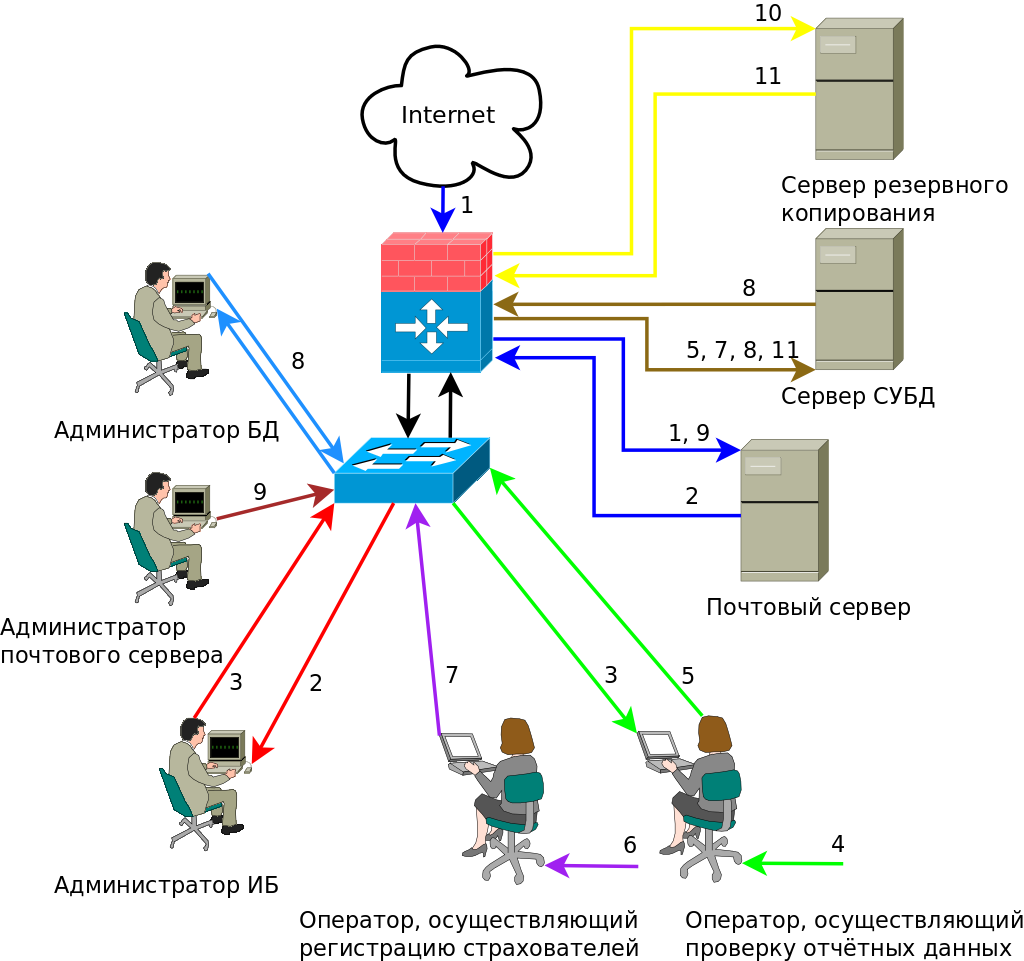
\includegraphics[width=\textwidth]{InfResurs}
  \caption{Схема информационных потоков и ИС фонда}
  \label{fig:infresurs}  
\end{figure}

\cleardoublepage

\section{Идентификация актуальных угроз для информационных ресурсов
  отделения фонда социального страхования}
\label{sec:2}

\subsection{Описание угроз защищаемым информационным ресурсам}

\point Во второй части курсовой работы необходимо идентифицировать наиболее
актуальные для информационных ресурсов фонда угрозы.

Разработка описания угроз защищаемым информационным ресурсам фонда
осуществляется на основе модели угроз из национального стандарта ГОСТ
Р ИСО/МЭК 15408.

\point Исходные перечень угроз:

\begin{itemize}
\item нарушение конфиденциальности защищаемой информации;
\item нарушение целостности защищаемой информации.
\end{itemize}

\point Уровнями информационно-технологической инфраструктуры фонда, по
которым следует локализовать каждый вид угроз из заданного перечня:

\begin{itemize}
\item уровень сетевых приложений, к которым можно отнести почтовые
  программные средства;
\item уровень операционных систем.
\end{itemize}

\point На уровне сетевых приложений можно выделить следующие угрозы:

\begin{itemize}
\item угроза внедрения в программу почтового сервера вредоносного кода;
\item угроза утечки аутентификационных данных сотрудников фонда;
\item угроза атаки на SSH-сервер;
\item уграза атаки на программу почтового сервера.
\end{itemize}

\point На уровне операционных систем можно выделить следующие угрозы:

\begin{itemize}
\item угроза внедрения в ОС программы-вируса;
\item угроза уничтожения или некорректной настройки критических файлов
  ОС администратором ИБ.
\end{itemize}

\point Угроза внедрения в программу почтового сервера вредоносного
кода, описанная в таблице может быть реализована по следующим двум
сценариям.

\point Злоумышленник, не имеющий отношения к отделению фонда, желает
получить конфиденциальную информацию, содержащуюся в отчётных данных
страхователей, для использования её в корыстных целях.

В связи с тем, что в отделении фонда социального страхования версии
программного обеспечения обновляются недостаточно часто, злоумышленник
может использовать ошибки его реализации, например, у некоторых
серверов в файле \texttt{/etc/aliases} присутствует строка
\texttt{decode: |/usr/bin/uudecode} автоматического запуска программы
\texttt{uudecode} для распаковки сообщений \texttt{UUE}.

Многие расшифровщики помещают раскодированный текст в файл, указанный
в заголовке \texttt{UUE}, допуская его перезапись без запроса
подтверждения от пользователя. Если, как часто и бывает, почтовый
сервер обладает наивысшими привилегиями, программа \texttt{uudecode}
унаследует их при запуске, а злоумышленник получает возможность
перезаписи любого файла в системе.

Например, он может внести в файл \texttt{/.forward} строку вида
\texttt{oot}, \texttt{root@somehost.org}~--- для организации
дублирования почты администратора на свой собственный адрес.

Далее начинает производиться несанкционированная пересылка писем,
приходящих на почтовый сервер, посторонним лицам по Интернет, тем
самым нарушается конфиденциальность важной информации. Вероятность
такого нападения высока. Масштаб прямого ущерба для
информационно-технологической инфраструктуры отделения фонда в данном
случае следует признать серьезным.

\point Программист-злоумышленник, не имеющий отношения к отделению
фонда социального страхования, обладающий детальными знаниями языков
программирования и принципов работы антивирусных программ, достигший
профессионального уровня в написании вредоносных программ-вирусов, с
целью умышленного причинения вреда пользователям сети Интернет для
повышения самооценки пишет новый компьютерный вирус, основанный на
уязвимости в реализации почтового сервера, заключающейся в возможности
выполнить код на почтовом сервере, используя неявную поддержку
конвейера в полях \texttt{MAIL FROM} и \texttt{RCPT TO}.

Например, команда языка \texttt{Perl} может не только открывать файл,
но и запускать его, если в имени присутствует символ <<|>>,
обозначающий вызов конвейера.

Уязвимость возникла из-за того, что версии программного обеспечения
обновляются недостаточно часто.

С использованием ошибки переполнения буфера, вирус начинает
модифицировать информацию в письмах, приходящих на почтовый сервер,
тем самым нарушая целостность важной информации. Вероятность такого
нападения высока. Масштаб прямого ущерба для
информационно-технологической инфраструктуры фонда в данном случае
следует признать серьезным;

\point Угроза утечки аутентификационных данных сотрудников фонда,
описанная в таблице может быть реализована следующему сценарию.

\point Администратор ИБ отделения фонда социального страхования,
имеющий опыт работы высокого профессионального уровня, детально
знающий принципы работы программы сервера баз данных, при отсутствии
системы работы с персоналом в организации, попав в состояние
нескорректированной вовремя психологической неустойчивости, возникшей
из-за возможного увольнения за прогул, хочет отомстить руководству
фонда.

Администратор ИБ, обладая всеми необходимыми средствами
администрирования на своём рабочем месте, решает опубликовать в
интернете пароли для доступа к почтовым ящикам всех сотрудников фонда
Таким образом происходит нарушение конфиденциальности
аутентификационной информации, которая может быть использована лицами,
не имеющими отношения к отделению фонда, для осуществления НСД к
письмам, приходящим на почтовый сервер отделения фонда социального
страхования.

Возможность такого нападения маловероятна, но масштаб прямого ущерба
для информационно-технологической инфраструктуры фонда следует
признать серьёзным.

\point Угроза атаки на \texttt{SSH}-сервер, описанная в таблице может
быть реализована по следующему сценарию.

\point Для доступа к почтовому серверу в отделении фонда используется
безопасное соединение с использованием сетевого протокола
\texttt{SSH}, позволяющий шифровать весь трафик, включая и
передаваемые пароли.

Администратор ИБ, не обладая необходимыми знаниями, совершил ошибки в
настройки \texttt{SSH}-сервера:

\begin{itemize}
\item не запретил удалённый \texttt{root}-доступ;
\item не изменил порт для доступа к \texttt{SSH}-серверу;
\item не ограничил список \texttt{IP}-адресов, с которых разрешен
  доступ;
\item использовал недостаточно надёжный пароль.
\end{itemize}

Таким образом, злоумышленник, не имеющий отношения к отделению фонда
социального страхования, который может не обладать высоким знаниями в
программировании и не знать деталей функционирования информационной
системы фонда, получает возможность получить привилегию пользователя
\texttt{root} на почтовом сервере. В результате этого может быть
нарушена конфиденциальность и целостность критической для
жизнедеятельности фонда информации~--- отчётных данных страхователей,
хранимых на почтовом сервере.

Возможность такого нападения высока и масштаб прямого ущерба для
информационно-технологической инфраструктуры отделения фонда следует
признать серьёзным.

\point Угроза атаки на программу почтового сервера, описанная в
таблице может быть реализована по следующему сценарию.

\point Злоумышленник, не имеющий отношения к отделению фонда
социального страхования, обладающий детальными знаниями языков
программирования и принципов работы межсетевых экранов, а также
имеющий большой опыт в их преодолении, с целью умышленного причинения
вреда отделению фонда для повышения самооценки производит сканирование
сетевых портов \texttt{TCP/UDP} серверов фонда с целью обнаружения
незащищенных.

Мотивом данного действия служит возможность хищения конфиденциальной
информации для использования ее в корыстных целях. В связи с тем, что
установленный в отделении фонда межсетевой экран не обеспечивает
необходимую защиту, при сканировании компьютерный взломщик с легкостью
обнаруживает незащищенные порты, после чего производит
несанкционированное подключение к почтовому серверу отделения через
Интернет и хищение конфиденциальной информации, находящейся в письмах,
которые приходят по электронной почте. Таким образом происходит
нарушение конфиденциальности важной информации. Вероятность такого
нападения высока. Масштаб прямого ущерба для
информационно-технологической инфраструктуры отделения фонда
социального страхования в данном случае следует признать серьезным.

Вероятность такого нападения высока. Масштаб прямого ущерба для
информационно-технологической инфраструктуры отделения фонда в данном
случае следует признать серьёзным.

\point Угроза внедрения в ОС программы-вируса, описанная в таблице
может быть реализована по следующим трём сценариям.

\point Создатели антивирусных программ, не имеющие отношения к
отделению фонда социального страхования, являющиеся опытными
программистами, достигшими профессионального уровня в написании
программ-антивирусов, обладающие детальными знаниями языков
программирования, с целью умышленного причинения вреда пользователям
сети Интернет пишут новый компьютерный вирус, способный преодолеть
существующие на текущий момент антивирусные защитные
системы. Антивирусная программа создается параллельно с этим вирусом.

Мотивом данного действия является явная коммерческая выгода для
создателей антивирусных программ, поскольку появление нового
неизвестного вредоносного кода вынуждает пользователей сети Интернет
покупать обновленные версии антивируса.

Ввиду того, что вирусные базы антивирусной программы в отделении фонда
социального страхования обновляются недостаточно часто, вышеописанный
вирус попадает в ИС фонда, после чего внедряется в системные и
загрузочные файлы операционных систем, под управлением которых
находится почтовый сервер и сервер БД. После внедрения вирус начинает
изменять системные и загрузочные файлы ОС. В результате этого в
процессе обработки происходит нарушение целостности БД, размещенной на
сервере БД и отчётных данных страхователей, размещённых на почтовом
сервере. Вероятность такого нападения высока. Масштаб прямого ущерба
для информационно-технологической инфраструктуры фонда в данном случае
следует признать серьёзным;

\point Программист-злоумышленник, не имеющий отношения к отделению фонда
социального страхования, обладающий детальными знаниями языков
программирования и принципов работы антивирусных программ, достигший
профессионального уровня в написании вредоносных программ-вирусов, с
целью умышленного причинения вреда пользователям сети Интернет для
повышения самооценки пишет новый компьютерный вирус, способный
преодолеть существующие на текущий момент антивирусные защитные
системы.

Вирус, проявивший себя в сети Интернет, обнаруживается специалистами
организаций, занимающихся разработкой антивирусных программ, после
чего для антивирусных программ в короткий срок выпускаются очередные
обновления, способные бороться с указанным вирусом.

Домашний компьютер администратора БД, не имеющий антивирусной защиты,
заражается вирусом типа <<\texttt{spyware}>>, копия вируса
перезаписывается на флеш-накопитель администратора.

Администратор БД подключает флеш-накопитель на своём
автоматизированном месте в отделении фонда социального страхования.

В связи с тем, что в отделении фонда вирусные базы антивирусной
программы обновляются недостаточно часто, вирус проникает в ИС фонда,
после чего внедряется в системные файлы операционных систем, под
управлением которых находится сервер БД и почтовый сервер. После
внедрения вирус начинает пересылку конфиденциальных данных о
страхователях злоумышленнику. В результате этого в процессе обработки
происходит нарушение конфиденциальности БД, размещенной на сервере БД,
отчётных данных страхователей, размещённых на почтовом
сервере. Вероятность такого нападения высока. Масштаб прямого ущерба
для информационно-технологической инфраструктуры отделения фонда в
данном случае следует признать серьёзным.

\point Программист-злоумышленник, не имеющий отношения к отделению
фонда социального страхования, обладающий детальными знаниями языков
программирования и принципов работы антивирусных программ, достигший
профессионального уровня в написании вредоносных программ-вирусов, с
целью умышленного причинения вреда пользователям сети Интернет для
повышения самооценки пишет новый компьютерный вирус, способный
преодолеть существующие на текущий момент антивирусные защитные
системы.

Вирус, проявивший себя в сети Интернет, обнаруживается специалистами
организаций, занимающихся разработкой антивирусных программ, после
чего для антивирусных программ в короткий срок выпускаются очередные
обновления, способные бороться с указанным вирусом. Но в связи с тем,
что в отделении фонда вирусные базы антивирусной программы обновляются
недостаточно часто, вирус проникает в ИС, после чего внедряется в
системные и загрузочные файлы операционной системы, под управлением
которой находится сервер БД. После внедрения вирус начинает изменять
системные и загрузочные файлы ОС.

В результате этого в процессе обработки происходит нарушение
целостности БД, размещенной на сервере БД. Вероятность такого
нападения высока. Масштаб прямого ущерба для
информационно-технологической инфраструктуры фонда в данном случае
следует признать серьёзным.

\point Угроза уничтожения или некорректной настройки критических
файлов ОС администратором ИБ, описанная в таблице может быть
реализована по следующим двум сценариям.

\point Администратор ИБ фонда, имеющий опыт работы высокого
профессионального уровня, детально знающий организацию операционной
системы, применяемой в ИС, и её функционирование, при отсутствии
системы работы с персоналом в организации, попав в состояние
нескорректированной вовремя психологической неустойчивости, возникшей
из-за возможного увольнения за прогул, хочет отомстить руководству
фонда и для демонстрации значимости своей работы руководству решает
умышленно нарушить целостность важной для ИС информации.

Используя как уязвимость доступность для редактирования системных
файлов ОС сервера БД, администратор ИБ производит их некорректное
редактирование.

В результате этого в процессе обработки происходит нарушение
целостности БД, размещенной на сервере БД.  Возможность такого
нападения маловероятна, но масштаб прямого ущерба для
информационно-технологической инфраструктуры отделения фонда
социального страхования следует признать серьёзным.

\point Администратор ИБ, имеющий опыт работы высокого
профессионального уровня, детально знающий организацию операционной
системы, применяемой в ИС, и ее функционирование, ввиду сильного
переутомления на рабочем месте, неумышленно производит некорректное
редактирование системных файлов ОС сервера БД.  В результате этого в
процессе обработки происходит нарушение целостности БД, размещённой на
сервере БД.  Возможность такого нападения маловероятна, но масштаб
прямого ущерба для информационно-технологической инфраструктуры
отделения фонда социального страхования следует признать серьёзным.

\subsection{Оценка рисков реализации угроз информационным ресурсам
  отделения фонда соцального страхования}

\point Точный прогноз актуальных угроз позволяет снизить риск
нарушения ИБ при минимизации затрат ресурсов организации. В процессе
анализа возможных и выявления актуальных для активов организации угроз
должен оцениваться риск, возникающий вследствие воздействия
определенной угрозы.

\point Первым этапом была произведена оценка риска причинения вреда
информационно-технологической инфраструктуре отделения фонда
социального страхования с учётом значений оценок возможностей
реализации угрозы безопасности, а также значений масштабов ущерба,
выявленных ранее при описании факторов угрозы.

\point На основе анализа возможности реализации каждой угрозы в
сочетании с масштабом ущерба для информационно-технологической
инфраструктуры, были выбраны определенные значения значимости риска с
учётом приведенных в таблице~\ref{tab:risk}. При этом были учтены
результаты, полученные в процессе формирования описания ИС, угроз и
сценариев реализации угроз на предыдущих этапах выполнения курсовой
работы.

\begin{table}[h]
\caption{Значимость риска, исходя из сочетания возможности нападения и масштаба ущерба}
\label{tab:risk}
\small
\begin{tabular}{|p{4cm}|p{2.5cm}|p{2.5cm}|p{2.5cm}|p{2.5cm}|}
\hline
\multirow{2}{4cm}{Возможность нападения} & \multicolumn{4}{c|}{Масштаб
ущерба}\\\cline{2-5}
& Катастрофиче\-ский~--- 4 & Значитель\-ный~--- 3 & Серьёзный~--- 2 &
Незначитель\-ный~--- 1 \\\hline
Частое~--- 6 & 24 & 18 & 12 & 6 \\\hline
Возможное~--- 5 & 20 & 15 & 10 & 5 \\\hline
Случайное~--- 4 & 16 & 12 & 8 & 4 \\\hline
Маловероятное~--- 3 & 12 & 9 & 6 & 3 \\\hline
Неправдоподобное~--- 2 & 8 & 6 & 4 & 2 \\\hline
Невозможное~--- 1 & 4 & 3 & 2 & 1 \\\hline
\end{tabular}
\end{table}
\normalsize

\point После этого полученное число для каждой угрозы было соотнесено
с интервалом на качественной шкале, форма которой показана в
таблице~\ref{tab:risk_scal}. Далее была составлена сводная таблица
значимости риска реализации угроз с точки зрения нанесения ущерба
информационно-технологической инфраструктуре, которая приведена в
таблице~\ref{tab:res_risk}.

\begin{table}[h]
  \caption{Качественная шкала значимости риска реализации угрозы}
  \label{tab:risk_scal}
\small
  \begin{tabular}{|c|c|c|c|}
    \hline
    Параметры & \multicolumn{3}{c|}{Интервалы шкал}\\\hline
    Балльные оценки &  24-9 & 8-4 & 3-1 \\\hline
    Качественные оценки & Высокая & Средняя & Низкая \\\hline
  \end{tabular}
\end{table}
\normalsize

\begin{table}[h]
  \caption{Сводная таблица значимости риска реализации угроз для информационно-технологической инфраструктуры отделения фонда социального страхования}
  \label{tab:res_risk}
\small
  \begin{tabular}{|p{2.5cm}|p{7cm}|p{2cm}|p{2cm}|}
    \hline
    \multicolumn{2}{|p{9.5cm}}{Угрозы по уровням инфраструктуры} &
    \multicolumn{2}{|p{5cm}|}{Значимость риска реализации угроз}\\\cline{3-4}
    \multicolumn{2}{|p{9.5cm}|}{} & Балльная оценка & Качественная оценка\\\hline
    \multirow{7}{2.5cm}{Уровень сетевых приложений} & Угроза внедрения в программу почтового сервера вредоносного
    кода & 12 & В \\\cline{2-4}
    & Угроза утечки аутентификационных данных сотрудников фонда & 6 &
    C \\\cline{2-4}
    & Угроза атаки на SSH-сервер & 12 & В \\\cline{2-4}
    & Угроза атаки на программу почтового сервера & 12 & В
    \\\hline
    \multirow{5}{2.5cm}{Уровень операционных систем} & Угроза
    внедрения в ОС программы-вируса & 12 & В \\\cline{2-4}
    & Угроза уничтожения или некорректной настройки критических файлов
  ОС администратором ИБ & 6 & С \\\hline
  \end{tabular}
\end{table}
\normalsize

\point Вторым этапом оценки риска, является анализ влияния реализации
угрозы на различные аспекты деятельности отделения фонда социального
страхования.  В отличие от оценки, даваемой на предыдущем этапе и
связанной в основном с оценкой технических последствий реализации
угрозы, на данном этапе во внимание принимается возможное влияние
реализации угрозы на деятельность отделения фонда.

\point Оценка рисков реализации угроз на уровнях сетевых приложений и
ОС инфраструктуры ОФСС была проведена с помощью заполнения матрицы
оценки риска.

\point Реализация угрозы нарушения целостности или конфиденциальности
информации путем внедрения в программму почтового сервера вредоносного
кода не приведет к серьёзным денежным потерям для отделения фонда
социального страхования, соответственно уровень риска денежной потери
следует принять низким. Уровень риска потери производительности в
данном случае высокий, так как нарушение целостности отчётов о работе
страхователей, полученных программой почтового сервера, приведёт к
некорректности результатов последующей работы ОФСС за длительный
период времени, что в свою очередь приведёт к необходимости
многократно повторять свои служебные обязанности персоналом
ОФСС. Уровень риска затруднения деятельности в данном случае также
высокий, так как нарушение конфиденциальности отчётов о работе
страхователей, полученных программой почтового сервера, приведёт к
серьезного подрыву доверия страхователей к отделению фонда социального
страхования.

\point Реализация угрозы нарушения конфиденциальности информации из-за
утечки аутентификационных данных сотрудников фонда не приведет к
серьёзным денежным потерям для ОФСС, соответственно уровень риска
денежной потери следует принять низким. Уровень риска потери
производительности в данном случае также низкий, так как реализация
данной угрозы не потребует дублирования усилий персонала отделения
фонда и не приведёт к недоступности бизнес-функций. Уровень риска
затруднения деятельности в данном случае следует принять высоким, так
как нарушение конфиденциальности аутентификационных данных для
подключения к \texttt{POP3}-серверу (\texttt{login},
\texttt{password}) может быть использовано лицами, не имеющими
отношения к отделению фонда, для осуществления НСД к письмам,
приходящим на почтовый сервер, что, в свою очередь, приведет к
серьёзному подрыву доверия страхователей к отделению фонда.

\point Реализация угрозы нарушения целостности или конфиденциальности
информации путем атаки на сервер \texttt{SSH} через Internet не
приведет к серьёзным денежным потерям для отделения фонда,
соответственно уровень риска денежной потери следует принять
низким. Уровень риска потери производительности в данном случае
средний, так как нарушение целостности отчётов о работе страхователей,
полученных программой почтового сервера, приведет к некорректности
результатов последующей работы ОФСС за короткий промежуток времени,
что в свою очередь приведет к необходимости продублировать работу
сотрудников ОФСС за это время. Уровень риска затруднения деятельности
в данном случае следует принять высоким, так как нарушение
конфиденциальности отчётов о работе страхователей, полученных
программой почтового сервера, приведет к серьёзного подрыву доверия
страхователей к отделению фонда.

\point Реализация угрозы нарушения конфиденциальности информации путем
атаки на почтовый сервер через Internet не приведет к серьёзным
денежным потерям для отделения фонда, соответственно уровень риска
денежной потери следует принять низким. Уровень риска потери
производительности в данном случае также низкий, так как реализация
данной угрозы не потребует дублирования усилий персонала отделения
фонда и не приведёт к недоступности бизнес-функций. Уровень риска
затруднения деятельности в данном случае следует принять высоким, так
как нарушение конфиденциальности отчётов о работе страхователей,
полученных программой почтового сервера, приведет к серьёзного подрыву
доверия страхователей к отделению фонда.

\point Уровень риска денежной потери при реализации угрозы нарушения
целостности или конфиденциальности информации путем внедрения в ОС
программы-вируса следует принять средним, так как модификация
системных и загрузочных файлов операционных систем, под управлением
которых находятся АРМ и серверы, входящие в состав ИС, приведёт к
невозможности дальнейшей работы данных ОС. Уровень риска потери
производительности в данном случае высокий, так как нарушение
целостности системных и загрузочных файлов операционных систем, под
управлением которых находятся АРМ и серверы, входящие в состав ИС, к
остановке их работы на длительный период времени. Уровень риска
затруднения деятельности в данном случае следует принять низким, так
как реализация данной угрозы не приведёт к подрыву общественного
доверия к отделению фонда социального страхования.

\point Уровень риска денежной потери при реализации угрозы нарушения
целостности информации путем уничтожения или некоректной настройки
критических файлов ОС администратором ИБ следует принять средним, так
как модификация системных и загрузочных файлов операционных систем,
под управлением которых находятся АРМ и серверы, входящие в состав ИС,
приведёт к невозможности дальнейшей работы данных ОС. Уровень риска
потери производительности в данном случае высокий, так как нарушение
целостности системных и загрузочных файлов операционных систем, под
управлением которых находятся АРМ и серверы, входящие в состав ИС, к
остановке их работы на длительный период времени. Уровень риска
затруднения деятельности в данном случае следует принять низким, так
как реализация данной угрозы не приведет к подрыву общественного
доверия к отделению фонда социального страхования.

\point Для определения общего риска нарушения деятельности организации
от реализации каждой угрозы были использована
таблица~\ref{tab:risk_rasch}, а также качественная шкала из
таблицы~\ref{tab:risk_scal}. Результат представлен в
таблице~\ref{tab:matr_ocenki} приложения~\ref{AppendixB}.

\begin{table}[h]
  \caption{Таблица для расчета общего риска нарушения деятельности}
  \label{tab:risk_rasch}
\small
  \begin{tabular}{|p{1.5cm}|p{1cm}|p{1cm}|p{1cm}|p{1cm}|p{1cm}|p{1cm}|p{1cm}|p{1cm}|p{1cm}|}
    \hline
    \multirow{4}{1.5cm}{Риск денежной потери} &
    \multicolumn{9}{c|}{Риск потери производительности} \\\cline{2-10}
    & \multicolumn{3}{c|}{Низкий} & \multicolumn{3}{c|}{Средний} &
    \multicolumn{3}{c|}{Высокий} \\\cline{2-10} 
    & \multicolumn{3}{p{4cm}|}{Риск затруднения деятельности}
    & \multicolumn{3}{p{4cm}|}{Риск затруднения деятельности}
    & \multicolumn{3}{p{4cm}|}{Риск затруднения деятельности}
    \\\cline{2-10} 
    & Н & С & В & Н & С & В & Н
    & С & В \\\hline
    H & 2 & 3 & 4 & 6 & 7 & 8 & 10 & 11 & 12 \\\hline
    С & 7 & 8 & 9 & 11 & 12 & 13 & 15 & 16 & 17 \\\hline
    В & 13 & 14 & 15 & 17 & 18 & 19 & 21 & 22 & 23 \\\hline
  \end{tabular}
\end{table}



%%% Local Variables: 
%%% mode: latex
%%% TeX-master: "../TermWork_OPOIB"
%%% End: 

\newpage
\begin{center}
  \Large{\textbf{ЗАКЛЮЧЕНИЕ}}
\end{center}
\addcontentsline{toc}{section}{Заключение}

Текст заключения.
\newpage


\begin{thebibliography}{99}
\bibitem{1} Автор1~И.~О., Автор2~И.~О. Название первой книги. "--- М.:
Название первого издательства, 1999. "--- 543~с.
\bibitem{2} Автор3~И.~О., Автор4~И.~О. Название второй книги. "--- К.:
Название второго издательства, 1999. "--- 543~с.
\end{thebibliography}

\ESKDappendix{обязательное}{Приложение c текстом и формулами}

Формулы, помещаемые в приложениях, должны нумероваться отдельной
нумерацией арабскими цифрами в пределах каждого приложения с
добавлением перед каждой цифрой обозначения приложения, например
формула \eqref{tabwidth}.

Расчет ширины колонки таблицы можно выполнить по формуле:

\begin{equation}
\label{tabwidth}
W_\text{кол} = K \cdot W_\text{textwidth} - 2 \cdot W_\text{tabcolsep}
- N_\text{rule} \cdot W_\text{arrayrulewidth},
\end{equation}

\begin{ESKDexplanation}
\item[где ] $K$ "--- коэффициент ширины;
\item $W_\text{textwidth}$ "--- ширина текста на странице;
\item $W_\text{tabcolsep}$ "--- ширина промежутка между
вертикальной линией, отделяющей ячейку таблицы, и текстом ячейки;
\item $N_\text{rule}$ "--- число вертикальных линий отводимых на
ячейку (для внутренних ячеек $1$, для внешних $1{,}5$);
\item $W_\text{arrayrulewidth}$ "--- толщина вертикальной линии, что
отделяет ячейки.
\end{ESKDexplanation}

\ESKDappendix{обязательное}{Исходный код программы}

\lstinputlisting[caption = {seed.cpp}, label = {seed.cpp}]{./src/seed.cpp}

\newpage

%%% Local Variables: 
%%% mode: latex
%%% TeX-master: "../Term_Work"
%%% End: 

\ESKDappendix{обязательное}{Оценка рисков реализации угроз
  информационным ресурсам отделения фонда социального страхования}
\label{AppendixB}

\begin{sidewaystable}[h]
\small
  \begin{longtable}{|p{2.5cm}|p{1.5cm}|p{2cm}|p{2cm}|p{1.5cm}|p{1.5cm}|p{1.5cm}|p{1.5cm}|p{3cm}|p{2cm}|p{2cm}|}
    \caption{Описание угроз}
    \label{tab:appb} \\
    \hline
    \multicolumn{11}{|c|}{Угроза внедрения в программу почтового сервера программы-вируса}\\
    \multicolumn{11}{|c|}{Место локализации угрозы: почтовый сервер}\\\hline
    Уязвимость & Возмож\-ность нападения & Метод нападения & Объект
    нападения & Тип потери & Масш\-таб ущерба & Источник угрозы & Опыт &
    Знание & Доступные ресурсы & Возможная мотивация действий\\\hline
    \multirow{2}{3cm}{Несвоевре\-менное обновление вирусных баз антивирусной программы,
    версий ПО; наличие уязвимости типа «buffer overflow»
    Зона локализации уязвимости: ПО, относящееся к среде
    эксплуатируемых систем} & Частая & Несанк\-циони\-рован\-ная пересылка
  вирусом отчетов посторонним лицам по Интернет  &  Отчёты о работе страхователей,
  полученные программой почтового сервера & Конфи\-ден\-циаль\-ность & Серь\-ёз\-ный &
  Програм\-мист-зло\-умыш\-лен\-ник, не имеющий отношения к фонду & Профес\-сиональ\-ный уровень
  & Деталь\-ное знание принципов работы антивирусных программ; высокий
  уровень знания языков программирования & Персональ\-ный компьютер,
  наличие подключения к Интернет & Умышлен\-ное причинение вреда в
  корыстных целях\\\cline{2-11}
  & Частая & Исполь\-зова\-ние имеющейся уязвимости для искажения информации в
  письмах, приходящих на почтовый сервер & Отчёты о работе
  страхователей, полученные программой почтового сервера & Целос\-тность
  & Серьё\-зный & Програм\-мист-злоу\-мышлен\-ник, не имеющий отношения к
  отделению фонда & Профес\-сиональ\-ный уровень & Детальное знание
  принципов работы антивирусных программ; высокий уровень знания
  языков программирования & Персональ\-ный компьютер, наличие
  подключения к Интернет & Умыш\-лен\-ное причинение вреда для повышения
  самооценки \\\hline
  \end{longtable}
\end{sidewaystable}
\newpage

\begin{sidewaystable}[h]
Продолжение таблицы~\ref{tab:appb}
\small
  \begin{longtable*}{|p{2.5cm}|p{1.5cm}|p{2cm}|p{2cm}|p{1.5cm}|p{1.5cm}|p{1.5cm}|p{1.5cm}|p{3cm}|p{2cm}|p{2cm}|}
    \hline
    \multicolumn{11}{|c|}{Угроза утечки аутентификационных данных
      сотрудников фонда}\\
    \multicolumn{11}{|c|}{Место локализации угрозы: почтовый сервер}\\\hline
    Уязвимость & Возмож\-ность нападения & Метод нападения & Объект
    нападения & Тип потери & Масш\-таб ущерба & Источник угрозы & Опыт &
    Знание & Доступные ресурсы & Возможная мотивация действий\\\hline
    Отсутствие средств мониторинга за действиями
    администраторов. Зона локализации уязвимости: программное
    обеспечение, относящееся к среде эксплуатируемых систем и
    персонал ИС & Мало\-вероят\-ная & Адми\-нист\-ратор ИБ решает опубликовать в
    интернете пароли для доступа к почтовым ящикам всех сотрудников фонда
    &  Отчёты о работе страхователей, полученные программой почтового
    сервера  & Конфи\-ден\-циаль\-ность & Серь\-ёз\-ный &
    Адми\-нист\-ратор ИБ & Профес\-сиональ\-ный уровень
    & Деталь\-ное знание принципов работы программы почтового сервера
    & Не обязательны & Умышлен\-ное причинение вреда в
    целях мести\\\hline
  \end{longtable*}
\end{sidewaystable}

\newpage

\begin{sidewaystable}[h]
Продолжение таблицы~\ref{tab:appb}
\small
  \begin{longtable*}{|p{2.5cm}|p{1.5cm}|p{2cm}|p{2cm}|p{1.5cm}|p{1.5cm}|p{1.5cm}|p{1.5cm}|p{3cm}|p{2cm}|p{2cm}|}
    \hline
    \multicolumn{11}{|c|}{Угроза атаки на SSH-сервер}\\
    \multicolumn{11}{|c|}{Место локализации угрозы: почтовый сервер}\\\hline
    Уязвимость & Возмож\-ность нападения & Метод нападения & Объект
    нападения & Тип потери & Масш\-таб ущерба & Источник угрозы & Опыт &
    Знание & Доступные ресурсы & Возможная мотивация действий\\\hline
    Некорректная настройка SSH-сервера. Зона локализации уязвимости: программное
    обеспечение, относящееся к среде эксплуатируемых систем   &
    Частая &  Несанк\-циони\-рован\-ное подключение к почтовому серверу
    через Интернет и изменение информации в письмах, хищение
    конфиденциальной информации
    &  Отчёты о работе страхователей, полученные программой почтового
    сервера  & Конфи\-ден\-циаль\-ность, целос\-тность & Серь\-ёз\-ный &
    Компью\-терный взломщик, пользователь сети Internet, не имеющий
    отношения к фонду & Не имеет значения
    & Хорошее знание принципов работы SSH-сервера
    & Персо\-наль\-ный компьютер, наличие подключения к Интернет  & Умышлен\-ное причинение вреда в
    для повышения самооценки\\\hline
  \end{longtable*}
\end{sidewaystable}


\newpage

\begin{sidewaystable}[h]
Продолжение таблицы~\ref{tab:appb}
\small
  \begin{longtable*}{|p{2.5cm}|p{1.5cm}|p{2cm}|p{2cm}|p{1.5cm}|p{1.5cm}|p{1.5cm}|p{1.5cm}|p{3cm}|p{2cm}|p{2cm}|}
    \hline
    \multicolumn{11}{|c|}{Угроза атаки на SSH-сервер}\\
    \multicolumn{11}{|c|}{Место локализации угрозы: почтовый сервер}\\\hline
    Уязвимость & Возмож\-ность нападения & Метод нападения & Объект
    нападения & Тип потери & Масш\-таб ущерба & Источник угрозы & Опыт &
    Знание & Доступные ресурсы & Возможная мотивация действий\\\hline
    Некорректная настройка SSH-сервера. Зона локализации уязвимости: программное
    обеспечение, относящееся к среде эксплуатируемых систем   &
    Частая &  Несанк\-циони\-рован\-ное подключение к почтовому серверу
    через Интернет и изменение информации в письмах, хищение
    конфиденциальной информации
    &  Отчёты о работе страхователей, полученные программой почтового
    сервера  & Конфи\-ден\-циаль\-ность, целос\-тность & Серь\-ёз\-ный &
    Компью\-терный взломщик, пользователь сети Интернет, не имеющий
    отношения к фонду & Не имеет значения
    & Хорошее знание принципов работы SSH-сервера
    & Персо\-наль\-ный компьютер, наличие подключения к Интернет  & Умышлен\-ное причинение вреда в
    для повышения самооценки\\\hline
  \end{longtable*}
\end{sidewaystable}

\newpage

\begin{sidewaystable}[h]
Продолжение таблицы~\ref{tab:appb}
\small
  \begin{longtable*}{|p{2.5cm}|p{1.5cm}|p{2cm}|p{2cm}|p{1.5cm}|p{1.5cm}|p{1.5cm}|p{1.5cm}|p{3cm}|p{2cm}|p{2cm}|}
    \hline
    \multicolumn{11}{|c|}{Угроза внедрения в ОС программы-вируса}\\
    \multicolumn{11}{|c|}{Место локализации угрозы: автоматизированные рабочие места и серверы}\\\hline
    Уязвимость & Возмож\-ность нападения & Метод нападения & Объект
    нападения & Тип потери & Масш\-таб ущерба & Источник угрозы & Опыт &
    Знание & Доступные ресурсы & Возможная мотивация действий\\\hline
    \multirow{3}{2.5cm} {Несвоевре\-менное обновление вирусных баз
    антивирусной программы. Зона локализации уязвимости:
    программное обеспечение, относящееся к среде эксплуатируемых систем}
    &
    Частая &  \multirow{2}{2cm}{Изменение или уничтожение вирусом системных и загрузочных файлов ОС}
    &   \multirow{2}{2cm}{Системные и загрузочные файлы операционных
      систем, под управлением которых находятся АРМ и серверы}   & Целост\-ность & Серь\-ёз\-ный &
    Созда\-тели антивирусной программы
    & Профес\-сиональ\-ный уровень
    & Детальное знание принципов работы антивирусных программ; высокий уровень знания языков программирования
    & Штат опытных программистов;  наличие подключения к Интернет  &
    Коммерчес\-кая выгода\\\cline{7-11}
    &&&&&&Програм\-мист-злоумыш\-ленник, не имеющий отношения к фонду
    & Профес\-сиональ\-ный уровень
    & Детальное знание принципов работы антивирусных программ; высокий
    уровень знания языков программирования & Персональ\-ный компьютер,
    наличие подключения к Интернет & Умышлен\-ное причинение вреда для повышения самооценки\\\cline{3-11}
    &&Получение НСД к информации путем использования программ типа
    <<spyware>> & Системные и загрузочные файлы операционных систем,
    под управлением которых находятся АРМ и серверы &
    Конфи\-ден\-циаль\-ность & Серьёз\-ный & Програм\-мист-злоумы\-шленник,
    не имеющий отношения к фонду & Профес\-сиональ\-ный уровень &
    Детальное знание принципов работы антивирусных программ; высокий
    уровень знания языков программирования & Персональ\-ный компьютер,
    наличие подключения к Интернет & Хищение информации для
    использования ее в корыстных целях\\\hline
  \end{longtable*}
\end{sidewaystable}

\begin{sidewaystable}[h]
Продолжение таблицы~\ref{tab:appb}
\small
  \begin{longtable}{|p{2.7cm}|p{1.5cm}|p{2cm}|p{2cm}|p{1.5cm}|p{1.5cm}|p{1.5cm}|p{1.5cm}|p{3cm}|p{2cm}|p{2cm}|}
    \hline
    \multicolumn{11}{|c|}{Угроза уничтожения или некорректной настройки критических файлов ОС администратором ИБ}\\
    \multicolumn{11}{|c|}{Место локализации угрозы: автоматизированные рабочие места и серверы}\\\hline
    Уязвимость & Возмож\-ность нападения & Метод нападения & Объект
    нападения & Тип потери & Масш\-таб ущерба & Источник угрозы & Опыт &
    Знание & Доступные ресурсы & Возможная мотивация действий\\\hline
    \multirow{2}{3cm}{Доступность редактир-ния системных и загрузочных файлов 
      (config.sys, boot.ini). Зона локализации уязвимости: персонал ИС
      и программное обеспечение, относящееся к среде эксплуатируемых
      систем} & Малове\-роятная & Некоррек\-тное редактирование
    системных и загрузочных файлов и некорректное использование
    механизма восстановления ОС   &  Системные и загрузочные файлы
    операционных систем, под управлением которых находятся АРМ и
    серверы  & Целост\-ность & Серь\-ёз\-ный &
  Админи\-стратор ИБ & Профес\-сиональ\-ный уровень
  & Детальное знание принципов работы антивирусных программ и сетевых
  приложений & Не обязательны & Умышлен\-ное причинение вреда в
  целях мести\\\cline{11-11}
  &&&&&&&&&& Неумыш\-ленное причинение вреда ввиду переутомления на
  рабочем месте \\\hline
  \end{longtable}
\end{sidewaystable}
\newpage

\newpage

\begin{sidewaystable}[h]
  \begin{longtable}{|p{2.7cm}|p{6cm}|p{0.7cm}|p{0.7cm}|p{0.7cm}|p{0.7cm}|p{0.7cm}|p{0.7cm}|p{0.7cm}|p{0.7cm}|p{0.7cm}|p{0.7cm}|p{0.7cm}|p{0.7cm}|}
    \caption{Матрица оценки рисков нарушения деятельности организации}
    \label{tab:matr_ocenki} \\
    \hline
    \multicolumn{2}{|p{8.7cm}|}{Угрозы по уровням инфраструктуры} &
    \multicolumn{3}{p{2.1cm}|}{Риск денежной потери} &
    \multicolumn{3}{p{2.1cm}|}{Риск потери производительности} &
    \multicolumn{3}{p{2.1cm}|}{Риск затруднения деятельности} &
    \multicolumn{3}{p{2.1cm}|}{Общий риск} \\\hline
    \multirow{4}{3cm}{Уровень сетевых прило\-жений} &
    Угроза внедрения в программу почтового сервера вредоносного кода
    &&&Н&В&&&В&&&В&&\\\cline{2-14}
    & Угроза утечки аутентификационных данных сотрудников фонда
    &&&Н&&&Н&В&&&&С&\\\cline{2-14}
    & Угроза атаки на SSH-сервер
    &&&Н&&С&&В&&&&С&\\\cline{2-14}
    & Угроза атаки на программу почтового сервера
    &&&Н&&&Н&В&&&&С&\\\hline
    \multirow{4}{3cm}{Уровень ОС} &
    Угроза внедрения в ОС программы-вируса
    &&С&&В&&&&&Н&В&&\\\cline{2-14}
    & Угроза уничтожения или некорректной настройки критических файлов
    ОС администратором ИБ
    &&С&&В&&&&&Н&В&&\\\hline
  \end{longtable}
\end{sidewaystable}

%%% Local Variables: 
%%% mode: latex
%%% TeX-master: "../TermWork_OPOIB"
%%% End: 

\end{document}
